\section{Historia} 

%------------------------------------------------
\subsection{Antecedentes}

\begin{frame}
	\begin{alertblock}{}
		\justify
		La creación de la teoría de conjuntos se debe a una sola persona, Georg Cantor. Antes de ver ello, primero examinamos algunas contribuciones preliminares.
	\end{alertblock}
\end{frame}

\begin{frame}
\frametitle{Edad antigua y media}
La teoría de conjuntos tiene su origen en los razonamientos sobre el infinito, que datan desde la época griega.\\

\startchronology
[startyear=-500, stopyear=1650]
\chronoevent{-450}{Zenon} 
%
\chronoperiode{476}{1492}{Edad Media} 
\chronoevent{1638}{Galileo} 
\stopchronology
\end{frame}

\begin{frame}
\frametitle{Edad moderna}

El trabajo de Boole es el fundamento de la lógica informática.\\

\startchronology
[startyear=1840, stopyear=1880]
\chronoevent[textwidth=1.5cm]{1847}{Boole} 

\chronoevent[textwidth=1.5cm]{1851}{ ~~Bolzano } 

\chronoevent[]{1872}{Dedekind} 
\stopchronology

Dedekind publica su construcción formal de números reales y da una definición rigurosa de un entero.
\end{frame}

%------------------------------------------------
\subsection{La teoría ingenua de conjuntos.}

\begin{frame}
\frametitle{Georg Cantor}
\begin{figure}
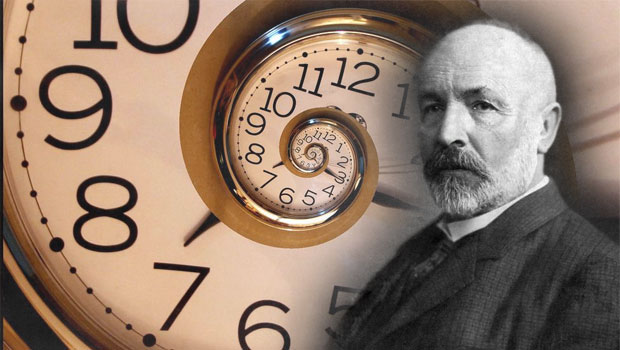
\includegraphics[width=1.\linewidth]{IMGS/cantor}
\end{figure}
\end{frame}

\begin{frame}
%\frametitle{Teoría de conjuntos de Cantor}

\justify
En 1874 Cantor publicó un artículo en el \textit{Crelle's Journal} ({\it \textcolor{blue}{Journal für die reine und angewandte Mathematik} }) 
el cual marca el nacimiento de la teoría de conjuntos.\\

\startchronology
[startyear=1870, stopyear=1910]
\chronoevent{1874}{Cantor} 
\chronoevent{1889}{Peano} 
\chronoperiode[startdate=false,stopdate=false,textwidth=3.5cm]{1897}{1902}{Paradojas;\endgraf 
1897: Burali-Forti;\endgraf
1899: Cantor;\endgraf
1901: Rusell} 
\stopchronology

\end{frame}

\begin{frame}
 \frametitle{La controversia}

\justify
Un segundo artículo fue presentado por Cantor en el \textit{Crelle's Journal} en 1878, pero la teoría de conjuntos ya se estaba convirtiendo en centro de la controversia. \\

Kronecker, quien estaba en la redacción de \textit{Crelle's Journal}, no estaba contento con las nuevas ideas revolucionarias contenidas en el documento de Cantor

\begin{block}{}
	\justify
	Cantor fue tentado a retirar el artículo, pero Dedekind persuadió a Cantor de no retirar su artículo y Weierstrass apoyó publicación.
\end{block}

\end{frame}

\begin{frame}
 \frametitle{El hotel de Hilbert}
  
 \begin{columns}[c] % La opción "c" especifica la alineación centrada vertical mientras la opción "t" es usada para alineación vertical superior

\column{.5\textwidth} % Columna izquierda con ancho ajustado al ancho de texto
\begin{figure}
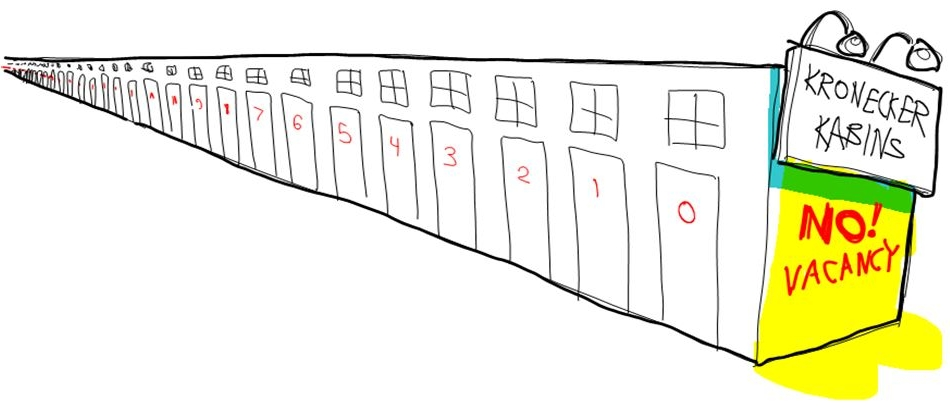
\includegraphics[width=1.1\linewidth]{IMGS/hilbert-hotel-L}
\end{figure}

\column{.5\textwidth} % Columna derecha con ancho ajustado al ancho de texto
\begin{figure}
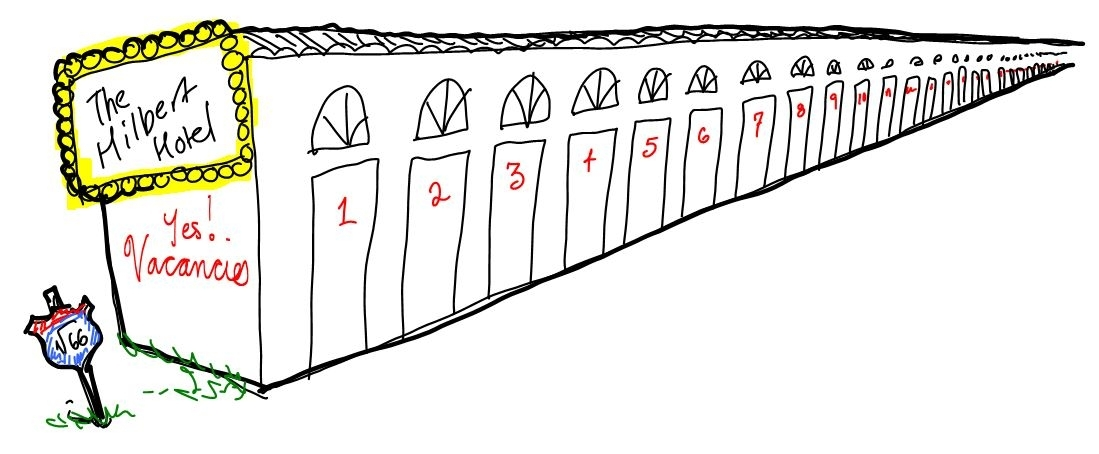
\includegraphics[width=1.1\linewidth]{IMGS/hilbert-hotel-R}
\end{figure}

\end{columns}

\vfill
\justifying
El hotel de Hilbert representa un acercamiento al entendimiento del infinito.
\end{frame}

\subsection{El discreto y el continuo}

\begin{frame}
 \frametitle{El conjunto de los números naturales}

\justify
Peano, en 1889, publica \textit{Arithmetices principia, nova methodo exposita} que donde expone los axiomas de Peano\\
 
\begin{block}{Axiomas de Peano}
 Existe un conjunto $N$, no vacío, y una función $s:N \to N$ de modo que se cumplen las siguientes propiedades:
 
 \pause
 \begin{enumerate}
  \item $s$ es inyectiva.
  \item $N\setminus s(N) = \{1\}$ %es un conjunto unitario, dicho elemento se denota $1$.
  \item Todo subconjunto de $N$ que contiene al $1$ y tiene la propiedad, $\forall n\in X, s(n)\in N$, no es otro sino $N$.
 \end{enumerate}
 \end{block}
\end{frame}

\begin{frame}
 \frametitle{El todo no es mayor que las partes}

\justify
Ya se tiene que $N$ es un modelo del conjunto de números naturales $\mathbb{N}$. En este modelo,
\begin{theorem}[Infinitud]
 Todo conjunto infinito tiene un subconjunto propio que se puede poner en correspondencia uno-uno a si mismo.
\end{theorem}

\pause
Es decir, todo conjunto infinito tiene una parte equipotente a si mismo.
\end{frame}

\begin{frame}
 \frametitle{El continuo}
 Dedekind logró construir los números reales ($\mathbb{R}$) a partir de los números racionales ($\mathbb{Q}$) usando la técnica de las \textit{cortaduras de Dedekind}.\\
 
 \pause
 {\color{red} Una pregunta que surge es si el infinito de los naturales y el infinito de los reales son iguales.}
 
 \pause
 \begin{theorem}[El continuo]
  No existe una biyección entre el conjunto de los naturales y el conjunto de los reales.
 \end{theorem}
\end{frame}


\begin{frame}
 \frametitle{La hipótesis del continuo}
 
 \begin{theorem}
  La potencia de un conjunto no es equipotente al conjunto.
 \end{theorem} 
 
 \pause
 \begin{theorem}
  El continuo es equipotente de a la potencia del discreto, es decir, 
  $$ \mathrm{card}\left( \mathbb{R} \right) = \mathrm{card} \left( P(\mathbb{N}) \right)$$
 \end{theorem}
 
 \pause
 \begin{alertblock}{Hipótesis del Continuo (HC)}
  Todo subconjunto infinito de $\mathbb{R}$ es o bien equipotente a $\mathbb{N}$ o bien equipotente a $\mathbb{R}$.
 \end{alertblock}
\end{frame}


%------------------------------------------------
\subsection{La paradoja del barbero}

\begin{frame}
 \frametitle{La paradoja del barbero}
 
 \begin{figure}
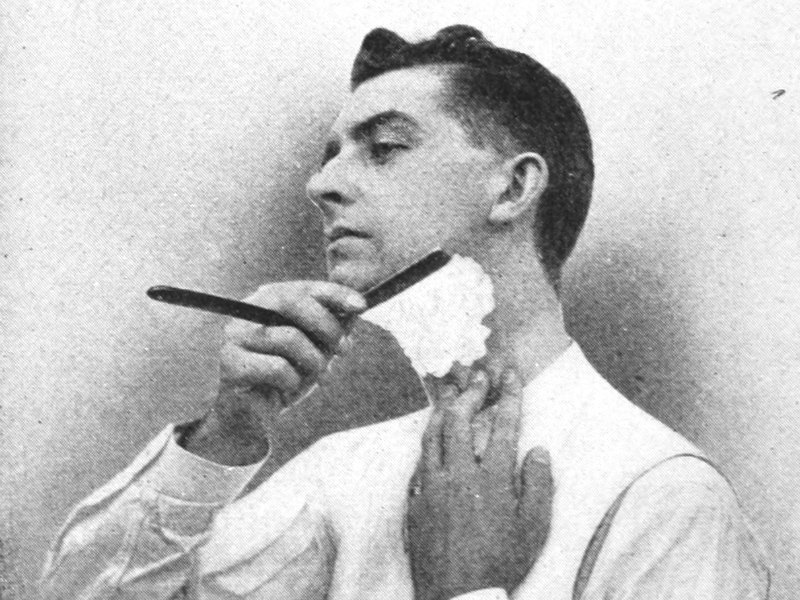
\includegraphics[width=0.8\linewidth]{IMGS/barbero}
\end{figure}
\end{frame}

\begin{frame}
 \frametitle{La paradoja de barbero}
 
\begin{block}{}
	Definamos un conjunto
	$$
	A = \{ X | ~X \text{no es elemento de} ~X\}
	$$
	Russell entonces se preguntó: 
	¿Es $A$ un elemento de $A$?
\end{block}

\pause
Tanto el supuesto de que $A$ es un miembro de $A$ y que $A$ no es un miembro de $A$ conllevan a una contradicción. 

\pause
\begin{center}
 ¡La propia construcción del conjunto parece dar una paradoja!
\end{center}
\end{frame}

